In this chapter we discuss the experimental evaluation of DyPyBench. We do so by answering the following questions:

% \textbf{RQ1:} How do the included test suites in Python projects within DyPyBench contribute to a dynamic benchmark?
\textbf{RQ1:} How the included test suites of Python projects make our benchmark dynamic ?

% \textbf{RQ2:} How efficient is our benchmark to generate (valid and good) training data for the neural models?
\textbf{RQ2:} Can our benchmark generate large and valid data to train neural models ?

% \textbf{RQ3:} How effective is DyPyBench in providing data to aid a comparison of static and dynamic call graph?
\textbf{RQ3:} Can we use our benchmark to compare static and dynamic analysis? 

\section{RQ1: How the Included Test Suites Make DyPyBench Dynamic ?}

DyPyBench provides a total of 45,086 test cases out of which 41,451 test cases pass and 429 fail.   
The number of test cases in each project varies from 1 to 10,552.
On average, each project has 902 test cases out of which 829 pass.  
The number of projects which have 0 failed test cases in DyPyBench is 31, whereas 13 others have failed tests between 1 and 10.
Figure \ref{fig:successful_tests} shows the percentage of passed test cases in all projects of DyPyBench.
We see that 41 projects have more than 90\% passed test cases, while 46 have 80\% or more passed test cases.
Overall, the pass percentage of 91.93\% is achieved for the test cases of all projects in DyPyBench.

\begin{figure}[ht]
    \centering
    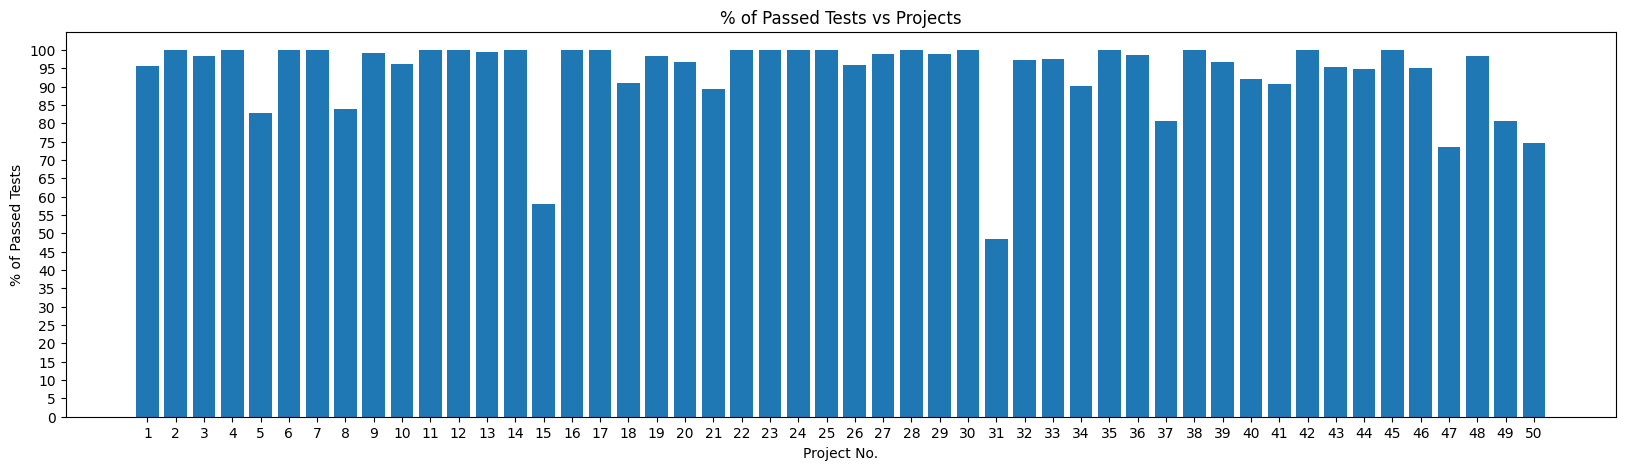
\includegraphics[width=1\linewidth]{figures/evaluation/perc_passed_tests.png}
    \caption[Passed Test Case Percentage ]{\label{fig:successful_tests}Percentage of Passed Tests in DyPyBench Projects.}
\end{figure}

The running time of test suite varies from 0.02 seconds and 1,362.86 seconds.
Figure \ref{fig:test_run_times} shows the run time of each project.
The total run time for all the projects in DyPyBench is 3,568.86 seconds.
On average, the running time per test case is 0.079 seconds, whereas the average time to run a test suite is 71.38 seconds. 
There are 39 projects which run the test suite within 50 seconds, whereas 4 projects have a run time greater than 200 seconds.
\begin{figure}[ht]
    \centering
    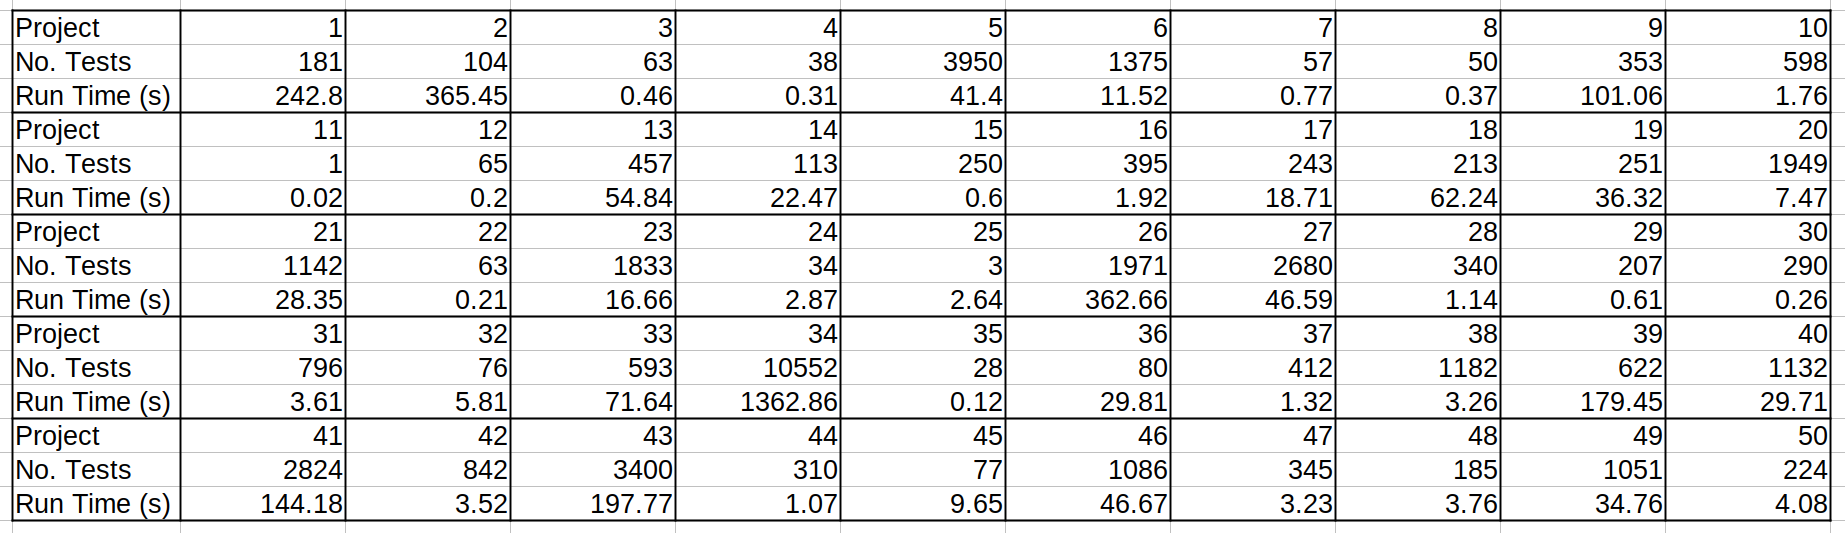
\includegraphics[width=1\linewidth]{figures/evaluation/tests_runtime2.png}
    \caption[Test Suite Run Time]{\label{fig:test_run_times}Test Suite Run Time in DyPyBench Projects.}
\end{figure}

\paragraph{Takeaway.} Overall, the included test suites make it easier to run the projects which is an important requirement to make a benchmark dynamic.
DyPyBench provides 45,086 test cases with a pass percentage of 91.93\%. 
With an average running time of 71.38 seconds for a single test suite, DyPyBench provides faster feedback and an increased productivity.
The availability of test suites make DyPyBench readily available for use, whereas the high pass percentage of test cases coupled with low run-time makes it dynamic in nature.

\section{RQ2: Can DyPyBench Provide Data for Neural Code Analysis ?}
DyPyBench contributes 547,830 new data points for LExecutor. 
This results in the model accuracy between 71.86\% and 93.67\% after training the model.

The new data points we collect are generated from 37 projects in our benchmark and amount to nearly 2.5 times the data points used by LExecutor.
Figure \ref{fig:Lex_projects_events} shows the data points from each project labelled with project number.
As can be seen from the Figure \ref{fig:Lex_projects_events}, the distribution of these data points vary from project to project.
This can be attributed to the number of files in each project that are instrumented. 
\begin{figure}[ht]
    \centering
    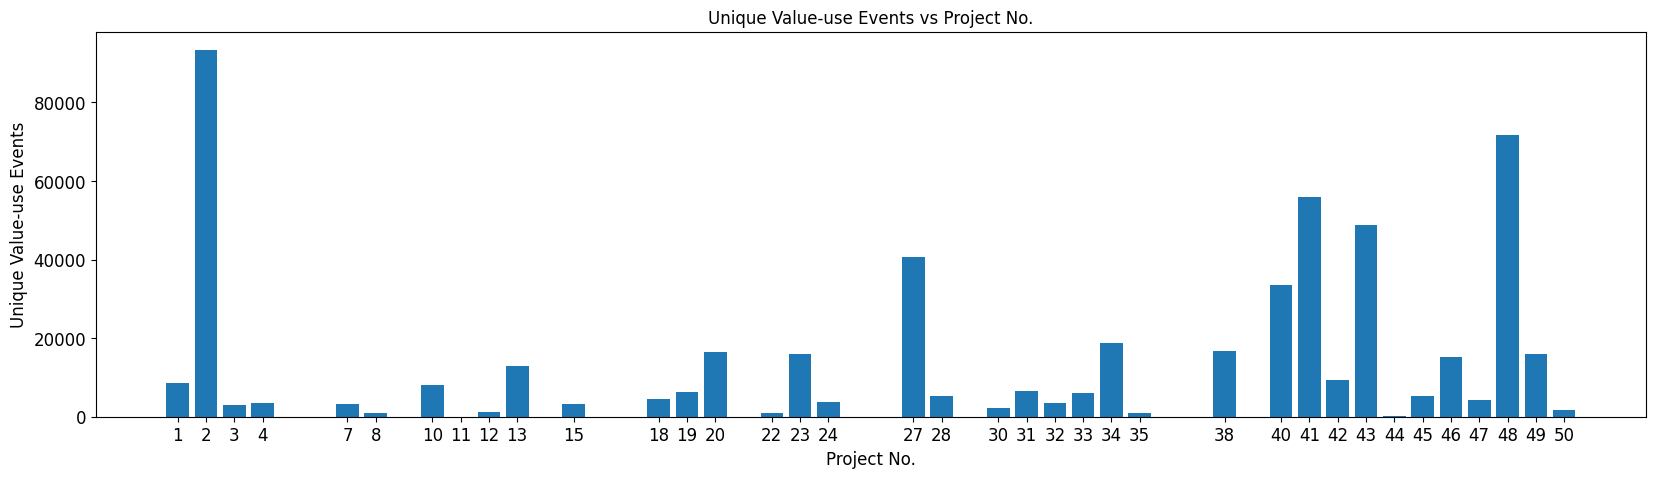
\includegraphics[width=1\linewidth]{figures/evaluation/lex_data_points.png}
    \caption[Unique Value-use Events]{\label{fig:Lex_projects_events}Unique Value-use Events in DyPyBench Projects}
\end{figure}

To evaluate the accuracy of the neural model based on the new data points, we perform a total of 6 experiments using different validation data and the abstraction modes.
Overall, we use 3 different validation data-sets.
First is a random split of 5\% from the data points we found with 37 projects in DyPyBench, second is the data-set provided by the LExecutor. This data-set has data points which were not for training the model.
Finally, the third data-set is the split from the new data points by projects. 6 projects were selected at random, which constitute nearly 5\% of the data points and these projects were excluded from 
training data-set.
For each of the validation data-set we perform 2 experiments, one with the abstraction mode as fine-grained while the other with coarse-grained as described before.

\begin{figure}[ht]
    \centering
    \subfigure[Fine-grained]{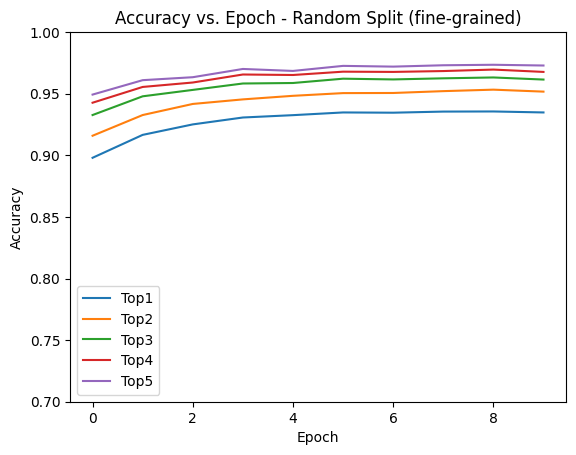
\includegraphics[width=0.4\linewidth]{figures/evaluation/lex_random_fine.png}}
    \subfigure[Coarse-grained]{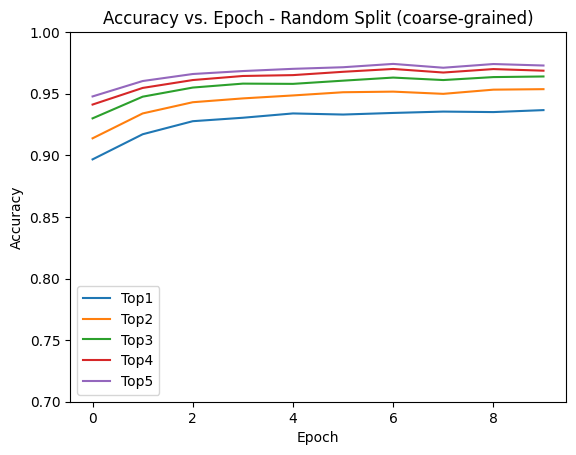
\includegraphics[width=0.4\linewidth]{figures/evaluation/lex_random_coarse.png}}
    \caption[Accuracy vs Epoch (Random Split)]{\label{fig:lex_random}Accuracy vs Epoch (Random Split) }
\end{figure}

Figure \ref{fig:lex_random} shows how the accuracy of the model varies with the number of epochs when the first validation data-set mentioned above is used.
Each line in the Figure \ref{fig:lex_random} shows the accuracy for top-n predictions for the same input variable.
As can be seen, the accuracy for top-5 is the best followed by top-4 and so on.
We mainly consider the accuracy of the first prediction, which starts at nearly 90\% and improves up to 93\% for both fine and coarse grained.

\begin{figure}[ht]
    \centering
    \subfigure[Fine-grained]{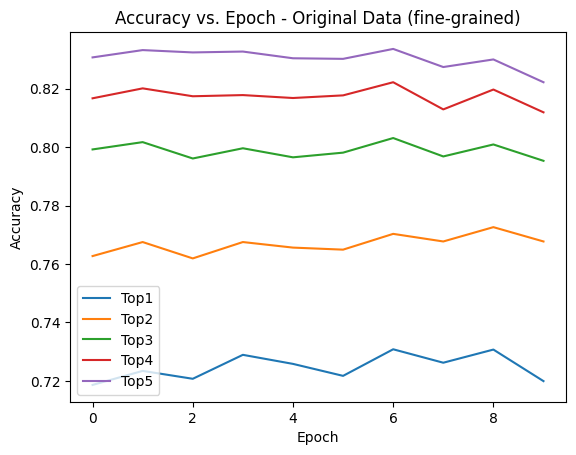
\includegraphics[width=0.4\linewidth]{figures/evaluation/lex_original_fine.png}}
    \subfigure[Coarse-grained]{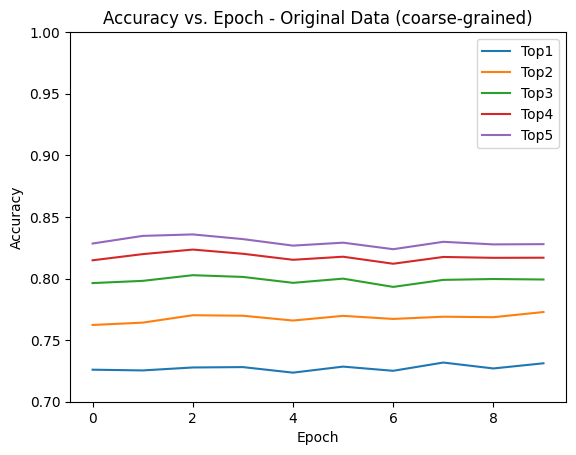
\includegraphics[width=0.4\linewidth]{figures/evaluation/lex_original_coarse.png}}
    \caption[Accuracy vs Epoch (Original Data)]{\label{fig:lex_original}Accuracy vs Epoch (Original Data) }
\end{figure}

Similarly, Figure \ref{fig:lex_original} shows the accuracy versus epoch for validation data-set used by the LExecutor.
As we can see in the Figure \ref{fig:lex_original}, the accuracy is lower than the previous experiments plunging down to 73\% in both cases of abstraction.
Finally, the Figure \ref{fig:lex_project} shows the accuracy versus epoch comparison for the third validation data-set mentioned above.
In this case, the accuracy ranges between the previous two experiments having the value of 85\% for both levels of abstraction.
For the first and second validation data-set, we get the best model in the 7th and 8th epoch.
However, for the third data-set the best model is found at the 4th epoch itself.
Since, the neural model we start with is a pre-trained model, the accuracy range we found is similar to the one specified by LExecutor.
\begin{figure}[ht]
    \centering
    \subfigure[Fine-grained]{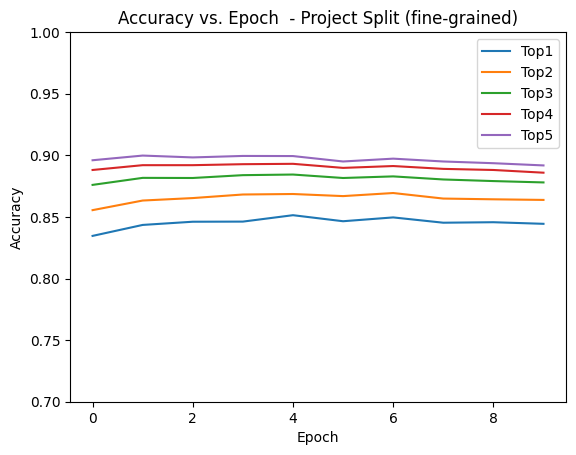
\includegraphics[width=0.4\linewidth]{figures/evaluation/lex_project_fine.png}}
    \subfigure[Coarse-grained]{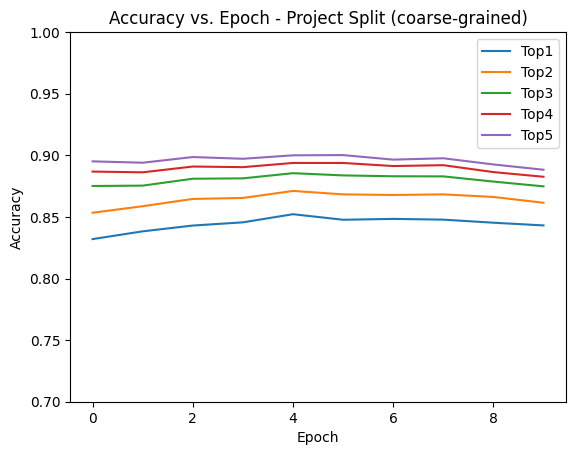
\includegraphics[width=0.4\linewidth]{figures/evaluation/lex_project_coarse.png}}
    \caption[Accuracy vs Epoch (Project Split)]{\label{fig:lex_project}Accuracy vs Epoch (Project Split) }
\end{figure}

\paragraph{Takeaway.} The quantity and quality of data is an important aspect for training neural network models. The higher quantity does not always guarantee the quality of data.
DyPyBench, provides projects which generates 547,830 data points for LExecutor, which results in a large quantity of data.
The quality of these data points is calculated based on the effect on accuracy.
The data points collected from DyPyBench, provide an accuracy in the range 71.86\% and 93.67\% for Top-1 predictions, which resonates with the accuracy provided by LExecutor without our data points.
Overall, DyPyBench is a good and valid data generator for neural analysis as it provides large quantity of good quality data.   

\section{RQ3: Can DyPyBench be Used to Compare Static and Dynamic Call Graphs ? }

DyPyBench provides 10,799 key data points from DynaPyt and PyCG combined for comparison of call graphs.
These key data points refer to the callers and are generated from 20 projects in DyPyBench.
From the above, 6,060 data points belongs to PyCG, and 4,739 are from PyCG.
With a manual verification of these data points, we find that PyCG provides a key for every entry in the list of callees, resulting in a higher number of keys in PyCG output.
However, when we compare the key data points in DynaPyt with PyCG there are no matches found.
Manually checking the this provides us the insight that the keys in PyCG have starting point as the root of the project while those in DynaPyt start from the root of the benchmark.
We fix this issue, by replacing the keys in DynaPyt with the appropriate values.
After the above fix, we get 3,147 key data points present in both.
66.41\% of keys in DynaPyt match with PyCG, while 51.93\% in PyCG are present in DynaPyt.
Figure \ref{fig:caller counts}, shows the distribution of the keys amongst DynaPyt and PyCG.
\begin{figure}[ht]
    \centering
    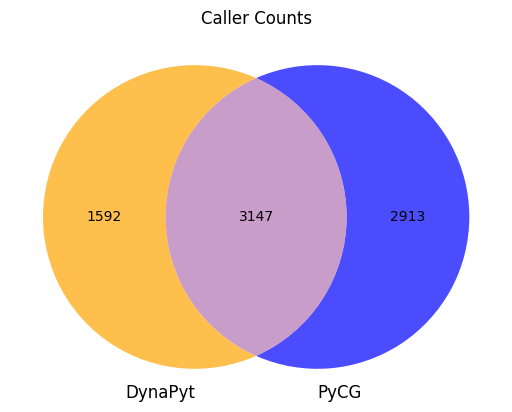
\includegraphics[width=0.5\linewidth]{figures/evaluation/callercounts.png}
    \caption[Distribution of Callers]{\label{fig:caller counts}Distribution of Callers }
\end{figure}
\begin{figure}[ht]
    \centering
    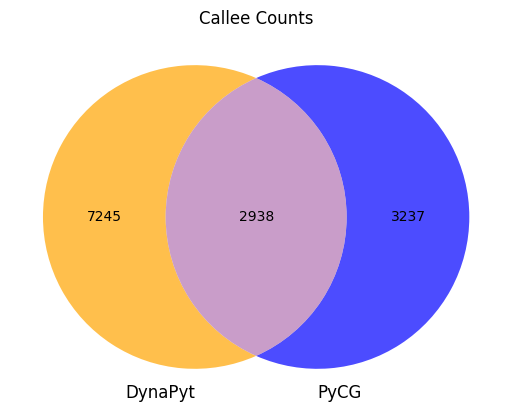
\includegraphics[width=0.5\linewidth]{figures/evaluation/calleecounts.png}
    \caption[Distribution of Callees]{\label{fig:callee_counts}Distribution of Callees}
\end{figure}

Next, we compare the number of value data points, which represent the callees.
We only compare the callees which are a part of the matching callers or keys.
There are a total of 16,493 value data points provided by DyPyBench for comparison, out of which 10,318 belong to DynaPyt and 6,175 to PyCG.% of callees for the same callers
The high number of values from DynaPyt is due to multiple callee entries of the same function, but from a different object.
PyCG cannot detect callees based on objects since, it generates the call graphs from static analysis.
Another factor that we saw from the manual inspection was the callee entries in DynaPyt for some private functions which PyCG is not able to provide. 
A direct string comparison of the value data points in DynaPyt with PyCG shows a match of 1,691 values.
This match contributes to 16.38\% match from DynaPyt and 27.38\% from PyCG.
With further manual verification, we find that certain data points essentially representing the same values do not match with a direct string comparison.
Figure \ref{fig:unmatched_value_strings} shows the differences of string in value data points from DynaPyt and PyCG.
\begin{figure}[ht]
    \centering
    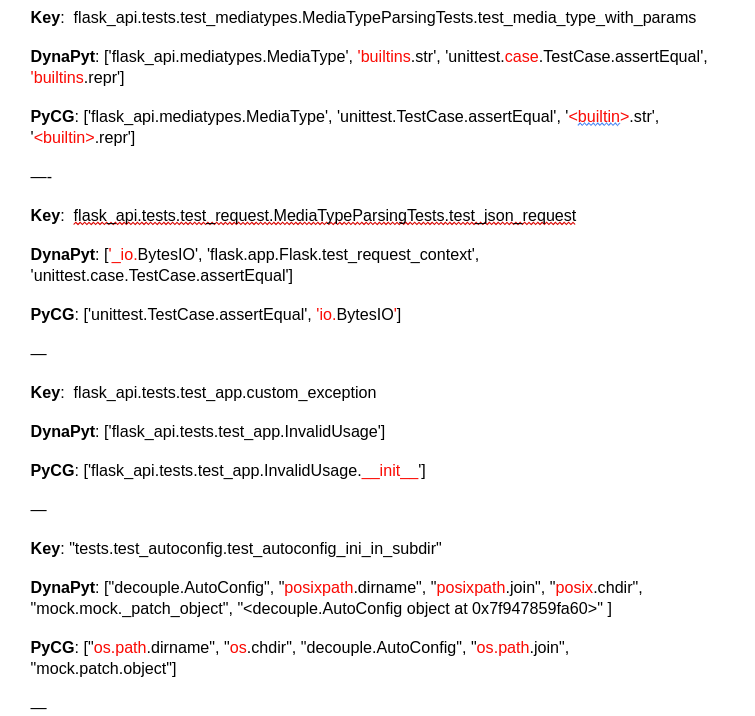
\includegraphics[width=0.8\linewidth]{figures/evaluation/string_compare.png}
    \caption[Unmatched Same Callees]{\label{fig:unmatched_value_strings}Unmatched Same Callees }
\end{figure}

Since the callees shown above are essentially the same, we include these in our comparison.
The number of matches in the value data points is now increased to 2,938, which significantly increases the percentage contribution of PyCG matches to 47.58\% and DynaPyt to 28.47\%. 10182
As mentioned before, DynaPyt contains multiple entries for callees with different objects, we remove duplicate entries of some of callees with similar patterns.
Firstly, we replace the pattern \verb|<decouple.AutoConfig object at 0x7f94786106a0>| by \textit{decouple.AutoConfig} and pop the duplicate entries of \verb|decouple.AutoConfig|.
Second, we replace the pattern \\\verb|BoundMethodWeakref(<tests.test_saferef._Sample1 object at 0x7f73338edb10>.x)| by \\\verb|BoundMethodWeakref(<tests.test_saferef._Sample1>.x)| and pop its duplicate entries.
The above modification of values data points leads to decrease in total data points to 16,358 which is a decrease of 136 callees from DynaPyt.
This results in a slight increase in the matching percentage of callees from DynaPyt to 28.85\%.
However, after manual verification of the callees we find patterns which should be included in the match but fail due to the module structure differences from DynaPyt and PyCG.
Figure \ref{fig:callee_counts} shows the distribution of the values amongst DynaPyt and PyCG for the matched keys.

\paragraph{Takeaway.} Static and dynamic analysis are important tools for code analysis.
A comparison of the two provides us an indication of how efficient is one over the other.
DyPyBench generates data for comparison of static and dynamic analysis of call graphs using DynaPyt and PyCG.
With more than 50\% matching callers from both frameworks, DyPyBench provides relevant data for comparison between the two.
A low percentage (28.85\%) of match for the callees provides us a deeper insight into execution flow of Python programs to compare the two analysis approaches.
Although, DyPyBench provides comparable data, there are certain limitations incorporated into the callee entries which impact the match percentage and need manual comparison of the two.
